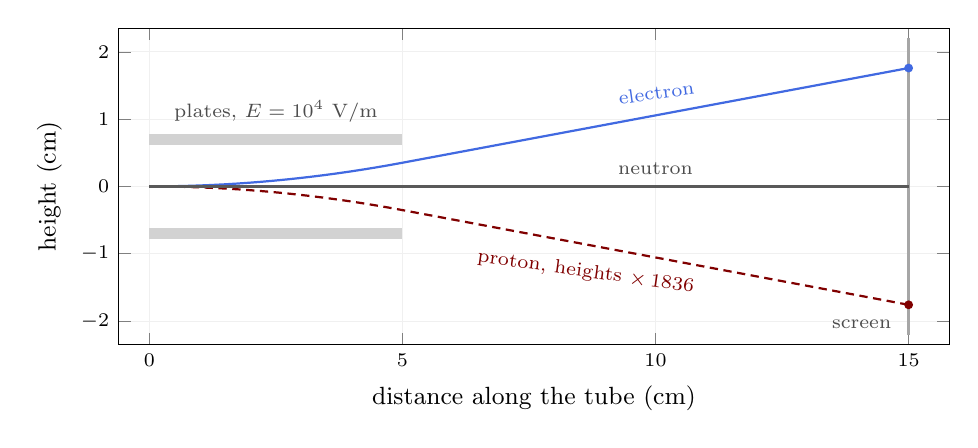
\begin{tikzpicture}
\begin{axis}[width=\textwidth, height=5.6cm, xmin=-0.6, xmax=15.8, ymin=-2.35, ymax=2.35,
  xlabel={distance along the tube (cm)}, ylabel={height (cm)}, xtick={0,5,10,15}, ytick={-2,-1,0,1,2},
  tick label style={font=\scriptsize}, label style={font=\small}, grid=major, grid style={gray!12}]
\fill[gray!35] (axis cs:0,0.62) rectangle (axis cs:5,0.78);
\fill[gray!35] (axis cs:0,-0.78) rectangle (axis cs:5,-0.62);
\node[font=\scriptsize, text=gray!60!black, anchor=south] at (axis cs:2.5,0.8) {plates, $E = 10^4$ V/m};
\draw[very thick, gray!70] (axis cs:15,-2.2) -- (axis cs:15,2.2);
\node[font=\scriptsize, text=gray!60!black, anchor=south east] at (axis cs:14.85,-2.25) {screen};
\addplot[RoyalBlue, thick] coordinates {(0.0000,0.0000) (0.2475,0.0009) (0.4950,0.0034) (0.7425,0.0078) (0.9900,0.0138) (1.2375,0.0215) (1.4850,0.0310) (1.7325,0.0422) (1.9800,0.0552) (2.2275,0.0698) (2.4750,0.0862) (2.7225,0.1043) (2.9700,0.1241) (3.2175,0.1457) (3.4650,0.1689) (3.7125,0.1939) (3.9600,0.2206) (4.2075,0.2491) (4.4550,0.2793) (4.7025,0.3111) (4.9500,0.3448) (5.0000,0.3518) (15.0000,1.7586)};
\addplot[Maroon, thick, densely dashed] coordinates {(0.0000,0.0000) (0.2475,-0.0009) (0.4950,-0.0034) (0.7425,-0.0078) (0.9900,-0.0138) (1.2375,-0.0215) (1.4850,-0.0310) (1.7325,-0.0422) (1.9800,-0.0552) (2.2275,-0.0698) (2.4750,-0.0862) (2.7225,-0.1043) (2.9700,-0.1241) (3.2175,-0.1457) (3.4650,-0.1689) (3.7125,-0.1939) (3.9600,-0.2206) (4.2075,-0.2491) (4.4550,-0.2793) (4.7025,-0.3111) (4.9500,-0.3448) (5.0000,-0.3518) (15.0000,-1.7586)};
\addplot[gray!70!black, thick] coordinates {(0.0000,0.0000) (0.2475,0.0000) (0.4950,0.0000) (0.7425,0.0000) (0.9900,0.0000) (1.2375,0.0000) (1.4850,0.0000) (1.7325,0.0000) (1.9800,0.0000) (2.2275,0.0000) (2.4750,0.0000) (2.7225,0.0000) (2.9700,0.0000) (3.2175,0.0000) (3.4650,0.0000) (3.7125,0.0000) (3.9600,0.0000) (4.2075,0.0000) (4.4550,0.0000) (4.7025,0.0000) (4.9500,0.0000) (5.0000,0.0000) (15.0000,0.0000)};
\fill[RoyalBlue] (axis cs:15,1.7586) circle (1.6pt);
\fill[Maroon] (axis cs:15,-1.7586) circle (1.6pt);
\node[font=\scriptsize, text=RoyalBlue, anchor=south east, rotate=8] at (axis cs:11,1.25) {electron};
\node[font=\scriptsize, text=Maroon, anchor=north east, rotate=-8] at (axis cs:11,-1.25) {proton, heights $\times\,1836$};
\node[font=\scriptsize, text=gray!60!black, anchor=south] at (axis cs:10,0.03) {neutron};
\end{axis}
\end{tikzpicture}
